\documentclass[conference]{IEEEtran}
\IEEEoverridecommandlockouts
% The preceding line is only needed to identify funding in the first footnote. If that is unneeded, please comment it out.
\usepackage{cite}
\usepackage{amsmath,amssymb,amsfonts}
\usepackage{algorithmic}
\usepackage{graphicx}
\usepackage{textcomp}
\usepackage{xcolor}
\def\BibTeX{{\rm B\kern-.05em{\sc i\kern-.025em b}\kern-.08em
    T\kern-.1667em\lower.7ex\hbox{E}\kern-.125emX}}
\begin{document}

\title{Cognitive Radios}

\author{\IEEEauthorblockN{Andrei Tumbar}
\IEEEauthorblockA{\textit{Computer Engineering}}
\and
\IEEEauthorblockN{Jacob LaPietra}
\IEEEauthorblockA{\textit{Computer Engineering}}
}

\maketitle

\begin{abstract}
Cognitive radios are a solution implemented for wireless networking that intelligently detect in-use radio channels in real-time. By utilizing machine learning, cognitive radios may infer the usage context of the user and therefore be able to optimize large scale networks. Paths between receiver and transmitter can therefore be optimized dynamically based on real-time usage.
\end{abstract}

\section{Theory}

Wireless communication will utilize bands within the electromagnetic spectrum. With the exception of the industrial, scientific, and medical (ISM) bands, a user will need a license from their country's government to use the radio band. Researchers have been looking for ways that unlicensed users may utilize licensed radio bands without disturbing licensed users \cite{b1}. In the United States, the Federal Communications Commission (FCC) manages the use of the radio frequency bands to licensed users. Cognitive radios (CR) are a key technology able to leverage new transmitters that can dynamically change their operating band. This allows unlicensed users to fill in white space on the licensed bands allowing for less congestion overall and more efficient use of the spectrum \cite{b2}.

\begin{figure}[htbp]
\centerline{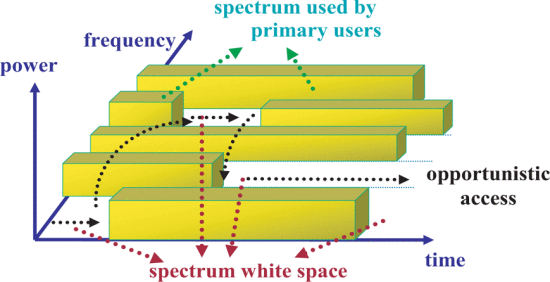
\includegraphics[width=8cm]{theory.png}}
\caption{Band sharing between primary and secondary users.}
\label{fig}
\end{figure}

Conventional wireless radio communication can become congested as the utilization of wireless space becomes over saturated with users. Conflicting wireless networks may conflict and degrade one another causing transmission issues on the channels in question. The Cognitive Radio (CR) is a developing technology that hopes to mitigate conflict over the wireless space by intelligently detecting and switching to bands with low utilization \cite{b1}.

CR looks to use more of the radio frequency spectrum dynamically. This means that a radio is able to choose between a spectrum of frequencies based on parameters such as channel utilization, noise, and energy efficiency. Priority level is another issue CR is able to accommodate. Most research toward implementing a priority system simply looks at a two tier system. Commonly dubbed the licensed or primary user (PU) and unlicensed or secondary user (SU). The SU must yield to a PU attempting to utilize the same channel. Use cases for this include things like emergency services, low-utilization safety critical devices such as autonomous vehicles.

Primary users inside a wireless network are meant to stay untouched by secondary users. In the current network schema, primary users are the only users allowed to utilize certain bands. Secondary users are therefore limited to unlicensed bands such as the ISM bands. Research in \cite{b6} has shown that cognitive radios may provide better opportunistic use of TV UHF bands in the 400-800 MHz bands as well as the 3-10 GHz bands.

\section{Cognitive Spectrum Sensing}
Cognitive Radios rely on a crucial technology to make switching between unused bands efficient: cognitive spectrum sensing. The idea here is that a wireless network will include an array of sensors that can detect in-use bands. These sensors will communicate with network users to coordinate EM bands that are available. The sensors can work with one of several transmitter detection methods: matched filter detection, energy detection, and cyclostationary detection \cite{b5}.

\subsection{Matched Filter Detection}
Matched filter detection (MF) is considered the optimal detection method in terms of accuracy. MF involves demodulation of the carrier signal on the respective band. This requires some prior knowledge of the primary user signal type including modulation type as well as software defined features such as packet format. To make this viable, the cognitive radio would require a dedicated receiver for every primary user band \cite{b6}. 

This detection could however be viable if a signal does not need to operate on a large
number of frequencies. A limited number of receivers could be used to broaden the usecase of a conventional radio.


\subsection{Energy Detection}
Energy detection is a simplified heuristic when comparing to the matched filter approach. Here the amplitudes of the signals are averaged after a Fast-Fourier-Transform (FFT). The noise power levels must be known so that a proper threshold level may be chosen. Because energy detection does not know much beyond static noise levels, misevaulation is susceptible to changing noise levels. When comparing to the matched filter design, energy detection does not know anything about how the channel will be utilized and therefore must essentially guess if a signal is sent by a primary user or if its simply noise \cite{b6}.

There are methods to improve the accuracy of energy detection. Similar to the exposure time of a camera, increasing the integration time of the channel will reduce its susceptibility to noise levels. Furthermore, increasing the FFT resolution will help with narrow band signal detection \cite{b6}. Providing more information about a primary user's transmissions would also improve the accuracy of this method. This would help the sensor to detect patterns in the channel that would indicate transmissions.

\subsection{Cyclostationary Detection}

A cyclostationary process is a signal that has a high probability of varying with time. Using this idea, CD is able to detect man-made transmissions in the presence of noise more accurately than simply looking at the energy levels of an EM band \cite{b5}. This is most useful when dealing with bands that have higher levels of external interference. Man-made signals are usually encoded with a certain modulation technique such as BPSK, QPSK, or SQPSK. These modulation techniques have a distinct power and spectral utilization. CD is essentially a specialized form of energy detection in which certain features are detected in the RF spectrum.

Cyclostationary detection is hugely effective even in environments where the SNR is as low as -20dB \cite{b6}.

\begin{figure}[htbp]
\centerline{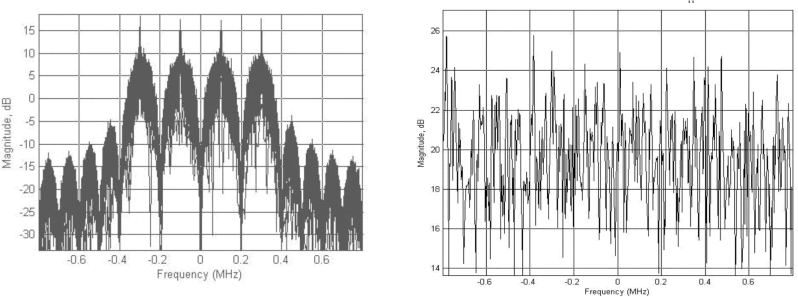
\includegraphics[width=8cm]{fsk_noise}}
\caption{Power spectrum density of 4-FSK modulation.}
\label{fig_fsk}
\end{figure}

Figure \ref{fig_fsk} \cite{b6} shows the power spectrum density of the 4-FSK modulation technique after an FFT in SNR=10dB (left) and SNR=-20dB. As previously stated, using a correlation function, cyclostationary detection is able to detect a signal in both of these situations. Note that the 4-FSK signals have a very distinctive power spectrum distribution function that can be correlated easily after a Fourier transform.

\section{Intelligent Cognition through Machine Learning}
So far, this paper has discussed the theory and operation of sensing for Cognitive Radios. A network of high quality sensors will provide the framework for a CR network, however, we are still missing the "cognitive" portion. Some CR network designs look to incorporate a learning engine to drive the decision making in optimizing network transmissions. Artificial Intelligence (AI) relies on a large amount of labelled data to help drive the AIs internal parameters to a local minima. The learning engine inside a cognitive radio network will try to predict the utilization based on trends of use by primary users over long period of time \cite{b7}.

There are many different learning algorithms used to optimize the CR including hidden Markov model, neural networks and genetic algorithms \cite{b7}. Every learning technique will have the same goal of maximizing channel capacity and efficiency. Because environments may vary from location to location, there is no direct mapping from sensory inputs to decision making outputs. This means that AI for CR will need to be trained for different environments and use cases.

\subsection{Modulation and Coding Rates}

Research in \cite{b7} has shown that varying the channel modulation and coding rates of a wireless channel can improve the channel capacity. Instead of performing a simple searching algorithm to find the peak point, a gradient search can be applied in which the searching algorithm will follow the slope of the multivariable function to its peak.

\begin{figure}[htbp]
\centerline{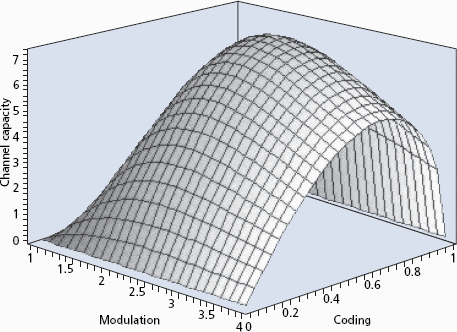
\includegraphics[width=8cm]{ml.png}}
\caption{Channel modulation and coding rate vs Channel Capacity}
\label{ml}
\end{figure}

Figure \ref{ml} shows an example of the resultant channel capacity as a function of modulation and coding rate. Because the gradient search method will simply settle on local extrema, \cite{b7} must assume that the channel capacity function is single peaked and concave down.

\subsection{Dynamic Spectrum Access}

The previous section discussed varying transmission parameters within the same channel to optimize channel capacity. While relevant to CR networks, this technique can be applied to conventional wireless networks without the need to switch between EM bands. A more important issue that machine learning hopes to solve is decision making in channel switching to avoid interference with primary users.

Secondary users decide which band to transmit on by choosing a band that has a low probabilty of being used by a primary user. To do this, a neural network could be used to compute the probability that a signal is transmitting on a certain line at a certain time. Using feedback from the sensory network, a neural network is able to adapt over time to better predict primary user channel use so that secondary users can avoid band switching \cite{b7}. Avoiding bands with high probablities is crucial as there is a significant time penalty to switching between bands.

\section{Applications}

Cognitive Radio Spectrum Sensing can be used for military and public safety. Use cases include battlefield surveillance, radiological and nuclear investigation and detection. In situations such as these, Cognitive Radio Sensing can scan a wide band of frequencies to detect areas where the band is in a higher level of use indicating a potential source of transmission.

\begin{figure}[htbp]
\centerline{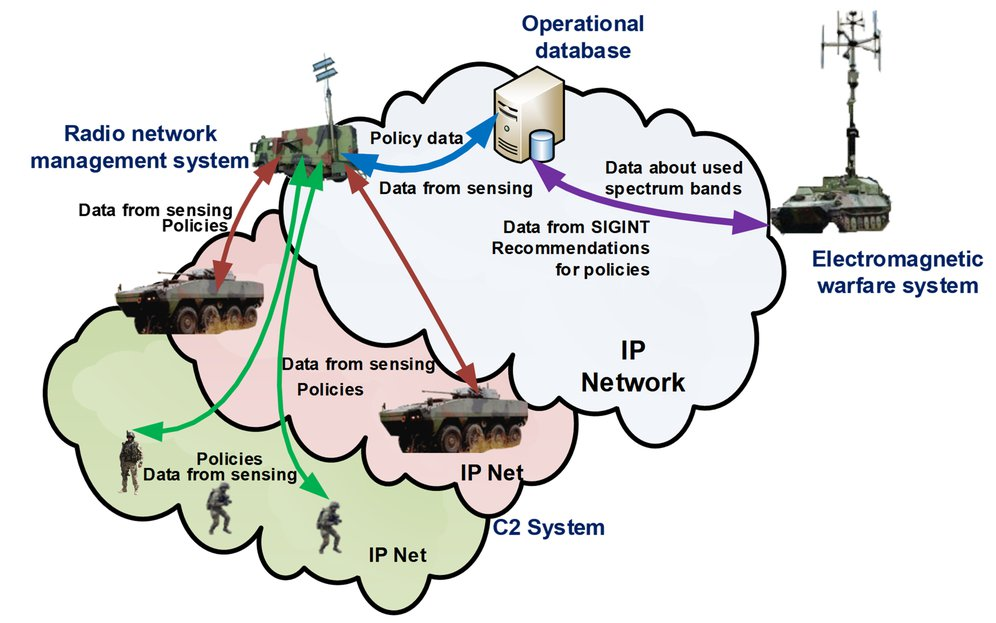
\includegraphics[width=8cm]{fig2.jpg}}
\caption{Radio frequency managemnt for millitary usage.}
\label{fig}
\end{figure}

\subsection{Healthcare}

In healthcare CR(Cognitive Radios) can be used to place sensors and monitoring devices for patients to be able to transmit medical information back to healthcare providers. In areas such as Nepal and India such devices are already in use where the ratio of healthcare providers to patients is relatively low \cite{b3}. The potential use of CR in healthcare is reduced since medical data is sensitive and precise so ensuring the collected data is accurate is difficult to verify.

\subsection{Household}

The use of CR in household appliances has potential uses since there is a increasing amount of devices in homes that use wireless technology to communicate with home monitoring and home automation systems, as well as entertainment devices. In these situations CR, would help with reducing interference between devices allowing for more reliable communications between devices.

\begin{figure}[htbp]
\centerline{
\includegraphics[width=8cm]{fig3.png}}
\caption{Small scale usage of cognitive radio technique.}
\label{fig}
\end{figure}

\subsection{Surveillance}

In real time surveillance applications, CR can be used in situations where there is traffic monitoring, environmental monitoring, disaster relief operations, as well as  inventory tracking. In these types of situations data collection is time and error sensitive, but the large amount of data collection devices can lead to congested wireless bands as well as link failures. In these applications CR can allow devices to find unused places in the spectrum for devices to transmit so that information can be passed along with less delay, instead of devices to wait for a optimal time for transmission to appear \cite{b4}.

\subsection{Power efficiency}

CR can be used when there is a cluster of radio based devices where lots of noise can be present in the spectrum. Radios will idle while there is too much interference to transmit or when the EM band has a high noise level. CR can switch these transmitters to better EM bands to reduce idle times or intelligently influence idle times via AI discussed previously. This approach reduces the necessary power consumption of the radios since they won't need to transmit as powerful of a signal to overcome the background noise. This is more helpful in clusters of radios since power usage can become more of an issue and sending messages without collisions can also cause radios to spend more power resending failed messages \cite{b2}.

\begin{figure}[htbp]
\centerline{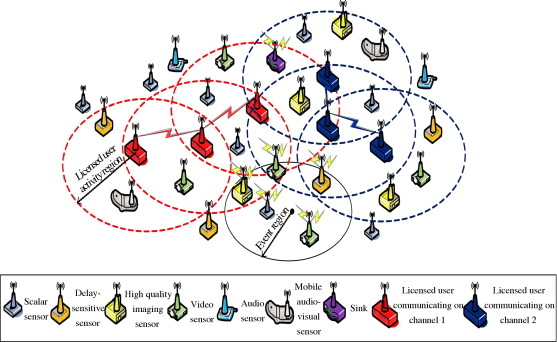
\includegraphics[width=8cm]{fig4.jpg}}
\caption{Small scale usage of cognitive radio technique.}
\label{fig}
\end{figure}

\section{Challenges}
One big challenge for CR is the hardware constraints of the radio sensors being used. Because of the many tasks the radios are responsible for there has not been specific definitions for how much computational power CRs should have. The use of AI has been proposed to be responsible for the detection and reconfiguration of the networks \cite{b2}. Because of the complicated overall system, a single solution has not been chosen for a standard yet \cite{b2}.

Another challenge is the manufacturing cost of CRs. Since CRs can be used in large networks of radios it would be ideal to have a low cost per radio however, due to the hardware needs of a CR radio, such as a more significant amount of memory, it is necessary to develop operational algorithms to reduce the needed computational power as well as system memory \cite{b2}. The development of more efficient radios will allow CR networks to be deployed for a cheaper cost.

Depending on the application, CRs will be deployed in very large numbers. These CR networks will need to communicate with other nodes among the network. As networks increase in size, it can be difficult to coordinate with each radio on an individual level \cite{b2}. It will be necessary to develop network protocols to help overcome the difficulty of managing such large networks.

Due to the environments that CRs will be deployed in, the wireless sensors need to be secure on a physical and software level. Not only can CR networks be tampered with by the falsification of data being sent to the radio, but the radios can be physically attacked due to the low human interactions with the majority of radios in a given network \cite{b2}. Because of these concerns, it is important to develop robust radios as well as robust protocols to prevent unauthorized access to the data within a CR network.

\section*{Conclusion}
Cognitive Radios have the potential to increase power efficiency, performance, and bandwidth utilization while keeping users with licensed EM spectrum access unaffected. One of the biggest advantages of CR is that it focuses purely on the secondary user. There is no requirement to change the current infrastructure for the licensed band user. This means companies and governments that need critical access to a specific radio frequency, will not need to update their technology to accommodate CR. Cognitive radios will simply open up access to more bands for unlicensed users who choose to integrate into the CR network. While the technology is still in its infancy, hardware and software advances have opened up avenues for further research to improve the viability of this technology.

\begin{thebibliography}{00}
\bibitem{b1} B. Wang and K. J. R. Liu, “Advances in Cognitive Radio Networks: A Survey,” IEEE Journal of selected topics in signal processing, vol. 5, no. 1, Feb. 2011.
\bibitem{b2} G. P. Joshi, S. Y. Nam, and S. W. Kim, “Cognitive Radio Wireless Sensor Networks: Applications, challenges and research trends,” Sensors (Basel, Switzerland), 22-Aug-2013. [Online]. Available: https://www.ncbi.nlm.nih.gov/pmc/articles/PMC3821336/. [Accessed: 20-Nov-2021].
\bibitem{b3} J. Mitola, “Cognitive Radio, An Integrated Agent Architecture for Software Defined Radio,” dissertation, 2000.
\bibitem{b4} H. Mehta, Recent Advances in Cognitive Radios. [Online]. Available: https://www.cse.wustl.edu/~jain/cse574-14/ftp/cr/index.html. [Accessed: 20-Nov-2021].
\bibitem{b5} R. Tandra and A. Sahai, "SNR Walls for Signal Detection," in IEEE Journal of Selected Topics in Signal Processing, vol. 2, no. 1, pp. 4-17, Feb. 2008, doi: 10.1109/JSTSP.2007.914879.
\bibitem{b6} D. Cabric, S. M. Mishra and R. W. Brodersen, "Implementation issues in spectrum sensing for cognitive radios," Conference Record of the Thirty-Eighth Asilomar Conference on Signals, Systems and Computers, 2004., 2004, pp. 772-776 Vol.1, doi: 10.1109/ACSSC.2004.1399240.
\bibitem{b7} C. Clancy, J. Hecker, E. Stuntebeck and T. O'Shea, "Applications of Machine Learning to Cognitive Radio Networks," in IEEE Wireless Communications, vol. 14, no. 4, pp. 47-52, August 2007, doi: 10.1109/MWC.2007.4300983.
\end{thebibliography}

\end{document}
